\documentclass[aspectratio=169]{../latex_main/tntbeamer}  % you can pass all options of the beamer class, e.g., 'handout' or 'aspectratio=43'
\usepackage{dsfont}
\usepackage{bm}
\usepackage[english]{babel}
\usepackage[T1]{fontenc}
%\usepackage[utf8]{inputenc}
\usepackage{graphicx}
\graphicspath{ {./figures/} }
\usepackage{algorithm}
\usepackage[ruled,vlined,algo2e,linesnumbered]{algorithm2e}
\usepackage{hyperref}
\usepackage{booktabs}
\usepackage{mathtools}

\usepackage{amsmath,amssymb}

\DeclareMathOperator*{\argmax}{arg\,max}
\DeclareMathOperator*{\argmin}{arg\,min}

\usepackage{amsbsy}
\newcommand{\vect}[1]{\bm{#1}}
%\newcommand{\vect}[1]{\boldsymbol{#1}}

\usepackage{pgfplots}
\pgfplotsset{compat=1.16}
\usepackage{tikz}
\usetikzlibrary{trees} 
\usetikzlibrary{shapes.geometric}
\usetikzlibrary{positioning,shapes,shadows,arrows,calc,mindmap}
\usetikzlibrary{positioning,fadings,through}
\usetikzlibrary{decorations.pathreplacing}
\usetikzlibrary{intersections}
\pgfdeclarelayer{background}
\pgfdeclarelayer{foreground}
\pgfsetlayers{background,main,foreground}
\tikzstyle{activity}=[rectangle, draw=black, rounded corners, text centered, text width=8em]
\tikzstyle{data}=[rectangle, draw=black, text centered, text width=8em]
\tikzstyle{myarrow}=[->, thick, draw=black]

% Define the layers to draw the diagram
\pgfdeclarelayer{background}
\pgfdeclarelayer{foreground}
\pgfsetlayers{background,main,foreground}

% Requires XeLaTeX or LuaLaTeX
%\usepackage{unicode-math}

\usepackage{fontspec}
%\setsansfont{Arial}
\setsansfont{RotisSansSerifStd}[ 
Path=../latex_main/fonts/,
Extension = .otf,
UprightFont = *-Regular,  % or *-Light
BoldFont = *-ExtraBold,  % or *-Bold
ItalicFont = *-Italic
]
\setmonofont{Cascadia Mono}[
Scale=0.8
]

% scale factor adapted; mathrm font added (Benjamin Spitschan @TNT, 2021-06-01)
%\setmathfont[Scale=1.05]{Libertinus Math}
%\setmathrm[Scale=1.05]{Libertinus Math}

% other available math fonts are (not exhaustive)
% Latin Modern Math
% XITS Math
% Libertinus Math
% Asana Math
% Fira Math
% TeX Gyre Pagella Math
% TeX Gyre Bonum Math
% TeX Gyre Schola Math
% TeX Gyre Termes Math

% Literature References
\newcommand{\lit}[2]{\href{#2}{\footnotesize\color{black!60}[#1]}}

%%% Beamer Customization
%----------------------------------------------------------------------
% (Don't) Show sections in frame header. Options: 'sections', 'sections light', empty
\setbeamertemplate{headline}{empty}

% Add header logo for normal frames
\setheaderimage{
	% 
\includegraphics[height=\logoheight]{figures/TNT_darkv4.pdf}
	
\includegraphics[height=\logoheight]{../latex_main/figures/luh_logo_rgb_0_80_155.pdf}
	% 
\includegraphics[height=\logoheight]{figures/logo_tntluh.pdf}
}

% Header logo for title page
\settitleheaderimage{
	% 
\includegraphics[height=\logoheight]{figures/TNT_darkv4.pdf}
	
\includegraphics[height=\logoheight]{../latex_main/figures/luh_logo_rgb_0_80_155.pdf}
	% 
\includegraphics[height=\logoheight]{figures/logo_tntluh.pdf}
}

% Title page: tntdefault 
\setbeamertemplate{title page}[tntdefault]  % or luhstyle
% Add optional title image here
%\addtitlepageimagedefault{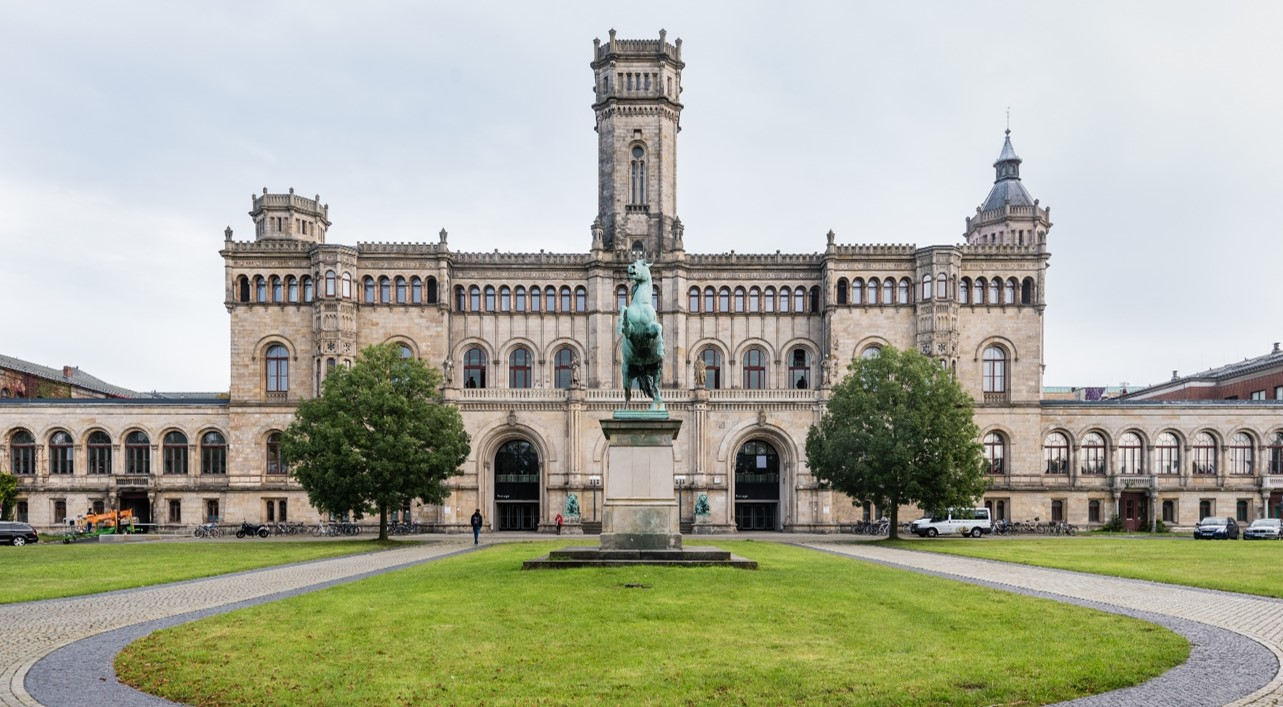
\includegraphics[width=0.65\textwidth]{figures/luh_default_presentation_title_image.jpg}}

% Title page: luhstyle
% \setbeamertemplate{title page}[luhstyle]
% % Add optional title image here
% \addtitlepageimage{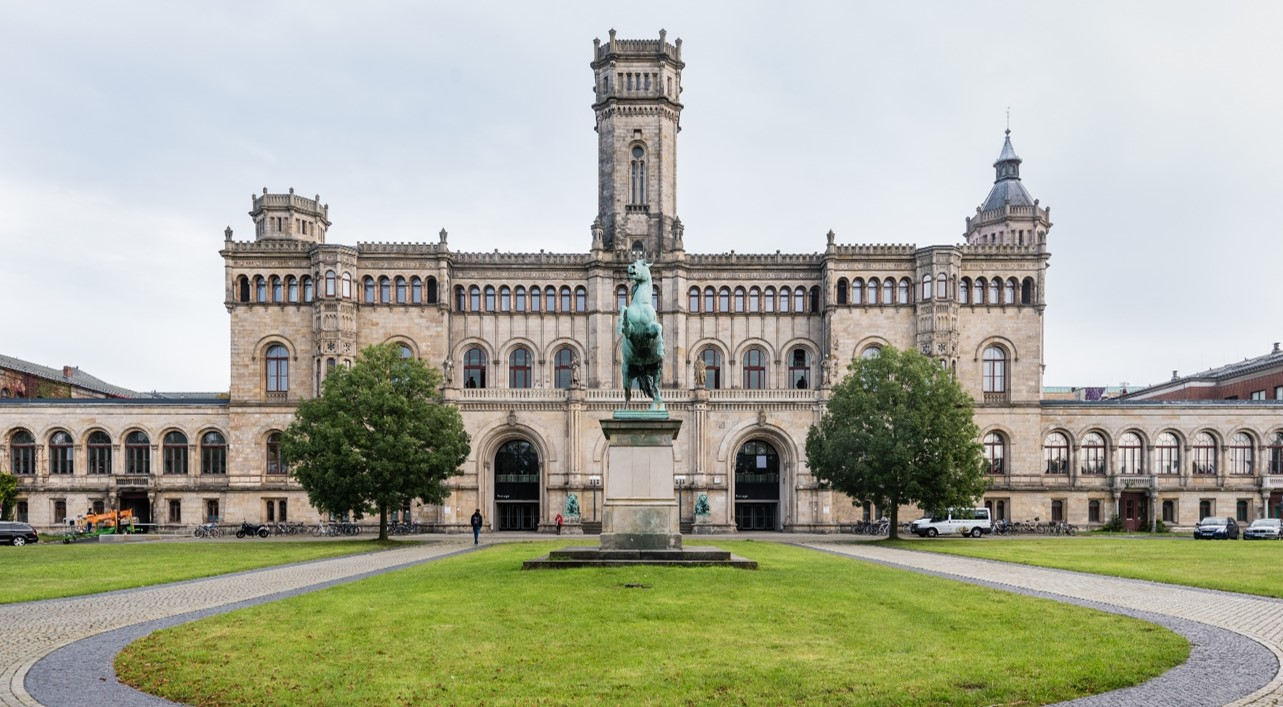
\includegraphics[width=0.75\textwidth]{figures/luh_default_presentation_title_image.jpg}}

\author[Abedjan \& Lindauer]{Ziawasch Abedjan \& Marius Lindauer\\[1em]
	
\includegraphics[height=\logoheight]{../latex_main/figures/luh_logo_rgb_0_80_155.pdf}\qquad
	
\includegraphics[height=\logoheight]{../latex_main/figures/DBIS_Kurzlogo.png}\qquad

\includegraphics[height=\logoheight]{../latex_main/figures/TNT_darkv4}\qquad

\includegraphics[height=\logoheight]{../latex_main/figures/L3S.jpg}	}
\date{Summer Term 2022; \hspace{0.5em} {
\includegraphics[height=1.5em]{../latex_main/figures/Cc-by-nc-sa_icon.svg.png}}; based on \href{https://ds100.org/fa21/}{[DS100]}
}


%%% Custom Packages
%----------------------------------------------------------------------
% Create dummy content
\usepackage{blindtext}

% Adds a frame with the current page layout. Just call \layout inside of a frame.
\usepackage{layout}


%%% Macros
%\renewcommand{\vec}[1]{\mathbf{#1}}
% \usepackage{bm}
%\let\vecb\bm

\title[Introduction]{DS: Inference for Modeling}
\subtitle{Bootstrap confidence intervals}

\graphicspath{ {./figure/} }
%\institute{}


\begin{document}
	
	\maketitle
	\begin{frame}{Confidence intervals}
	    \begin{itemize}
	        \item Intuition: Estimate an interval where we think the population parameter is, based on the center and variance of the estimator.
	        \item What does a P\% confidence interval mean?
	        \begin{itemize}
	            \item Imagine the following procedure:
	            \begin{itemize}
	                \item Take a sample from the population.
	                \item Compute P\% confidence interval for the true population parameter, somehow.
	            \end{itemize}
	            \item If we repeat this procedure many times, the population parameter will be in our interval P\% of the time, in the long run.
	        \end{itemize}
	    \end{itemize}
	\end{frame}
	
	
	\begin{frame}{Confidence intervals}
	    An estimator f exists in order to guess the value of an unknown parameter $\theta^*$.
        An estimator ci for a P\% confidence interval for f is a function that takes a sample and returns an interval. This interval will (ideally) contain $\theta^*$ for P\% of samples.
        \begin{columns}
            \begin{column}{.5\textwidth}
                    \begin{figure}
                        \centering
                        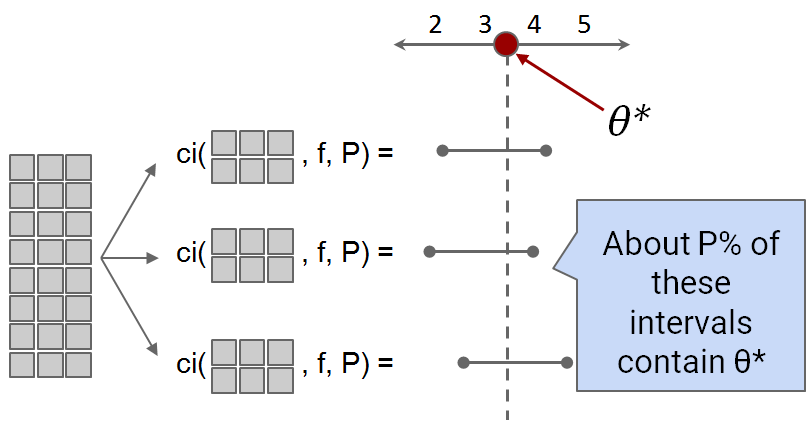
\includegraphics[scale=.35]{Bild8}
                    \end{figure}
            \end{column}
        
        
             \begin{column}{.5\textwidth}
             \\
             \bigskip
             \bigskip
                How do we compute ci(s,f,P)?
                    \begin{itemize}
                        \item Approximate the sampling distribution of f using the sample s.
                        \item Choose the middle P\% of samples from this approximate distribution.
                    \end{itemize}
            \end{column}
        
        \end{columns}
        
	\end{frame}
	
	
	
	\begin{frame}{Bootstrap confidence intervals}
	    An estimator ci for a P\% confidence interval for f is a function that takes a sample and returns an interval. This interval will (ideally) contain $\theta^*$ for P\% of samples.
	    \begin{figure}
	        \centering
	        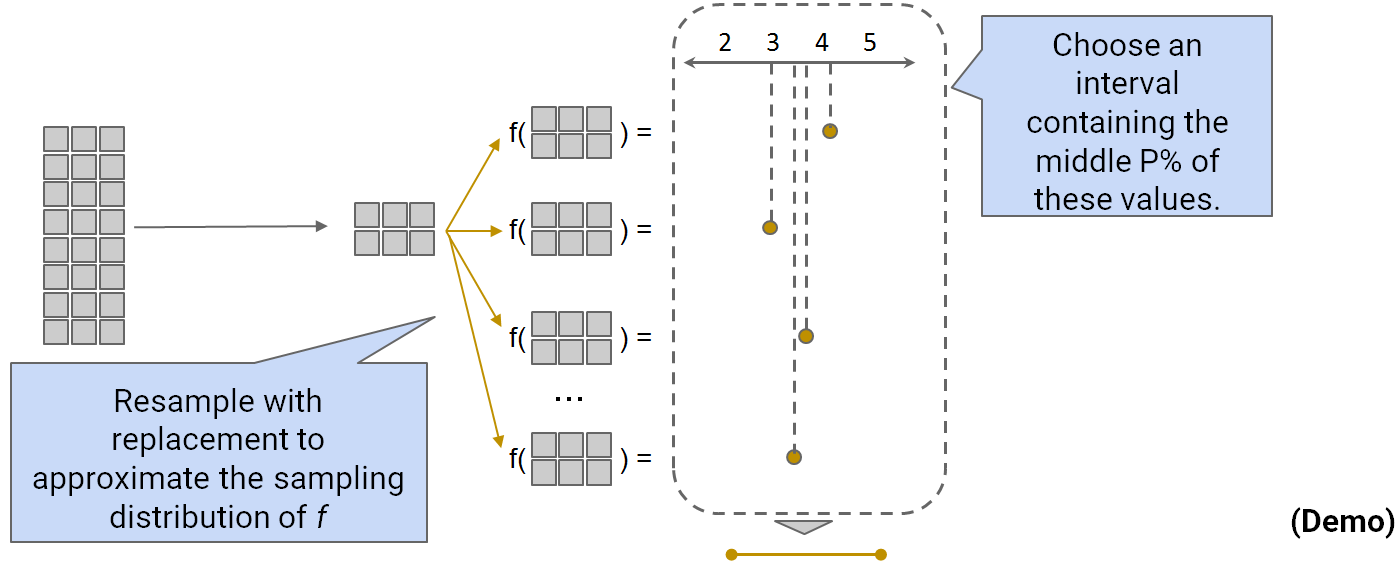
\includegraphics[scale=.35]{Bild9}
	    \end{figure}
	\end{frame}
	
	
	\begin{frame}{Confidence intervals}
	    \begin{itemize}
	        \item The confidence level is a statement about the procedure used to create our interval.
	        \item It is not the case that a 95\% confidence interval means “there is a 95\% chance that the population parameter is in our interval”.
	        \begin{itemize}
	            \item The population parameter is fixed.
	            \item Our interval is fixed. The population parameter is either in it, or it isn’t.
	            \item Nothing random here!
	        \end{itemize}
	        \item The confidence intervals we’ve created are sometimes called percentile bootstrap confidence intervals.
	        \begin{itemize}
	            \item There are other methods of creating confidence intervals.
	            \begin{itemize}
	                \item E.g. assume that the sampling distribution of your estimator is normal.
	            \end{itemize}
	        \end{itemize}
	    \end{itemize}
	\end{frame}
\end{document}